\documentclass[10pt, english, makeidx, a4paper, titlepage, oneside]{report}
% Geometry package
\usepackage[a4paper,width=150mm,top=30mm,bottom=25mm]{geometry}
\geometry{hmarginratio=1:1}

% General packages
\usepackage[utf8]{inputenc}
%\usepackage[italian]{babel}
\usepackage{hyperref}
\hypersetup{colorlinks=true}
\hypersetup{linkcolor=black}
\usepackage{siunitx}	% SI measurement units
\usepackage{amsmath}

% Graphics packages
\usepackage{xcolor}
\usepackage{multicol}
\usepackage{graphicx}
\usepackage{float}
\usepackage{hhline}
\usepackage{todonotes}
\usepackage{algorithmic}
\usepackage{subcaption}
\graphicspath{{images/}}

% Custom commands
%\newcommand{\rshift}{\ \texttt{>>}\ }
%\newcommand{\lshift}{\ \texttt{<<}\ }
% TITLE
\usepackage{tikz}
\usetikzlibrary{arrows,shapes,automata,petri,positioning,calc}

\usepackage{mdframed}
\usepackage{listings}
%\definecolor{codeBackground}{RGB}{250, 250, 250}
\definecolor{codeColor}{RGB}{50, 50, 50}
\definecolor{codeComment}{RGB}{90, 90, 90}
\definecolor{codeString}{RGB}{50, 175, 50}

\lstdefinestyle{lstStyle}{
    %backgroundcolor=\color{codeBackground},
    basicstyle=\ttfamily\footnotesize\linespread{0}\color{codeColor},
    commentstyle=\ttfamily\footnotesize\color{codeComment},
    keywordstyle=\bf\color{orange},
    stringstyle=\color{codeString},
    frame=tlbr,
    numbers=left,
    breaklines=true,
    showstringspaces=false,
    tabsize=2
}
\lstset{style=lstStyle}

\newcommand{\instr}{\texttt}


\title{
	{\Huge \textbf{Politecnico di Torino}}\\ \ \\
	{\Huge Integrated Systems Architectures} \\
	{\large Report for Lab 3}\\
	% {\small \url{https://github.com/levnikolaevicmiskyn/ISA/tree/main/lab2}} \\ \ \\
	{
\includegraphics[width=0.5\textwidth] {Politecnico_di_Torino.png}}
}
\author{
    {\Large \textsc{Group 12}}\\ \ \\
	Antonio Carlucci 276128\\
	Gabriele Perrone 269089\\
	Alessandro Scisca 276032
}
\date{} % Do not insert date
% START OF THE DOCUMENT
\begin{document}
\maketitle
\tableofcontents
\hypersetup{linkcolor=blue}
\newpage

\chapter{Universal Verification Methodology}
\section{Introduction}
The UVM is an open source verification standard consisting in a set of classes that extend the SystemVerilog language with advanced verification capabilities. A UVM testbench is made up of reusable components that are often an extension of the base classes already available and fit into a standardized testbench architecture. The object-oriented approach brings the verification task at an higher level of abstraction, which makes UVM a flexible and efficient environment. 

The general organization separates the verification domain from the DUT and its interface. Only the interface that closely interacts with the DUT needs to specify communication at the signal-level, while the remaining part that carries out most of the verification can operate at the transaction level (Transaction Level Model). 

\paragraph{TLM} Transactions are objects that model all the abstract features of communication between two objects. Interfaces for transaction-level communication are used in UVM to isolate the internal implementation of each component so that different components with the same interface can be swapped easily.
The elementary chunk of data exchanged in a transaction is an object of a custom class derived from \texttt{uvm\_sequence\_item}. This object includes all the variables, constraints and methods required to fully specify how data is structured and delivered in a given transaction. 

Instances of such sequence items exist in the testbench under analysis in two classes: \texttt{packet\_in} and \texttt{packet\_out}. They model the data generated by the sequencer and the packets collected at the DUT's output for checking/scoreboarding. In particular, \texttt{packet\_in} will deserve more attention since it describes the input sequence item as a couple of random integers $A$ and $B$ along with constraints that represent the properties that a valid input sequence must have.

Exchange of data happens, at the most simple level, between a producer component that \textit{puts} data on a port and a consumer with an associated export that \textit{gets} the transaction. The producer is the one that generates a transaction and sends it to its port using the \texttt{put} method. On the other hand, the consumer is expected to give an implementation of the \texttt{put} method, which is called whenever the producer wants to put data to its consumer. 

The converse operation on the consumer's side is to ask for a transaction from the producer. This is accomplished with the \texttt{get} method, called by the consumer and implemented in the producer.
For example, the \texttt{refmod} component contains both a get port and a put port objects, which allow to receive transactions from the agent and to send the result to the scoreboard.

\begin{lstlisting}[language = verilog, caption = Snippet from \textit{refmod.sv}]
packet_in tr_in;
packet_out tr_out;
uvm_get_port #(packet_in) in;
uvm_put_port #(packet_out) out;

virtual task run_phase(uvm_phase phase);
	[...]
	forever begin
		in.get(tr_in); // Get transaction from agent
		[...]
		out.put(tr_out); // Put transaction to the scoreboard
	end
endtask: run_phase
\end{lstlisting}

In this case the transactions are \textit{non-blocking}, they return instantaneously in the same delta cycle in which they are invoked.

\paragraph{Cycle} Every UVM object undergoes three distinct phases during a simulation run: all classes are required to give an implementation for these in the form of methods.
The \textbf{build phase} is where objects are created by means of the \texttt{create} method defined in the \texttt{uvm\_registry\_component} wrapper class. This way of creating objects is prescribed by the factory pattern, a paradigm drawn from object-oriented programming that is here employed to allow customization of objects through a configuration database rather than direct modification of the testbench code. Macros are used in every class to \textit{register} the object to the factory (as in line 2 of \ref{driver}). For instance, \texttt{uvm\_component\_utils} and \texttt{uvm\_object\_utils} are the macros for registering a new class type, respectively for classes derived from \texttt{uvm\_component} or \texttt{uvm\_object} classes\cite{sistenix}.

In the following snippet, the defult constructor simply calls its conterpart in the parent with default parameters to create an object whose default properties will be overridden later by means of the create method.

\begin{lstlisting}[language=verilog, label=driver]
class driver extends uvm_driver #(packet_in);
	`uvm_component_utils(driver) // Registration to the factory
	[...]
	// Constructor
	function new(string name = "driver", uvm_component parent = null);
		super.new(name, parent);
	endfunction
	
	// Build phase
	virtual function void build_phase(uvm_phase phase);
		super.build_phase(phase);
		assert(uvm_config_db#(input_vif)::get(this, "", "vif", vif));
	endfunction
\end{lstlisting}

The \textbf{connect phase} follows, where properly defined function create connection among testbench components by calling the \texttt{connect} method. As an example, the following snippet
shows the driver-sequencer connection and the link between the monitor and an \texttt{uvm\_analysis\_port} object.

\begin{lstlisting}[language=verilog, caption=Creation phase from the agent]
 virtual function void connect_phase(uvm_phase phase);
		super.connect_phase(phase);
		mon.item_collected_port.connect(item_collected_port); // Monitor connection
		drv.seq_item_port.connect(sqr.seq_item_export);       // Driver connection with sequencer
 endfunction
	\end{lstlisting}

Finally, the testbench is executed in the \textbf{run phase} and information are displayed in  the \textbf{report phase}.
\section{Architecture}
The testbench infrastructure used in this lab is freely provided by \textit{sistenix.com}. In the following, we report a brief overview of how different tasks are partitioned across components taking this particular implementation as a reference. This is still general, since the architecture is the one specified in the UVM standard \cite{uvm_book}, and can be expected to be essentially the same for all compliant implementations.

At the highest hierarchical level, verification tasks are performed in the \texttt{env} (\textit{environment}) entity, which instantiates the agents and the scoreboard.

\paragraph{Agent} The UVM standard defines the agent as the combination of a sequencer that produces the stimuli, a driver that communicates those stimuli to the DUT's interface and a monitor 
to gather the output data flow. This testbench includes a dedicated agent that operates in \textit{active} mode by driving the DUT's input interface. In particular, the \textit{sequencer} implements constrained random input generation at the transaction level, whose packet flow is then translated to bit-level signals by the \textit{driver}. These inputs must be forwarded to the scoreboard, this is accomplished by the \textit{monitor} that takes the signals at the driver's output back to the transaction level and puts them to the \textit{refmod}. 

A separate \textit{passive} agent collects the output data and it is made up of a driver and a monitor directly connected to the DUT's output interface.

\paragraph{Scoreboard} This component is in charge of verifying that the output results match those of a "golden" reference model for a given input. The behavioral description in the \textit{refmod} is an high level representation of the task that the DUT is supposed to perform: the design under test is correctly verified if it reproduces the refmod under all conditions.


\section{Constrained random input}
The goal of verification is, of course, to ensure the design correctness. Ideally, this should be checked throughout the whole space of possible input patterns. However, the combinations of legal input sequences are almost always too many to be tested in simulation, because it would simply take too long to complete. Hence, any practically feasible verification goal would consist in checking a small subset of all cases that is still representative of the whole set. Therefore, the target of a verification engineer is full coverage, which is a percentage that measures which fraction of all the interesting operating conditions have been verified. Complete coverage means that the design has been tested for all the conditions that are needed to be sure that it will work in every condition, including corner cases. 

Driving the DUT with a completely random input generator is not efficient since it might fail in exploring corner cases or even to give a fair representation on the input domain, with similar cases that might be tested multiple times needlessly. This hints that the sequence generation should directed by the engineer with suitable constraints. Given the importance of constrained random verification, there are specific tools in UVM that address this need. First of all, the keyword rand allows us to easily define a random variable, to which constraints may be attached to specify its range (the set of values that it can take) and its statistical distribution. For instance, the following code defines a random integer A in the interval [10,100] and a second variable B whose range, at any given time, is dependent on A.
\begin{lstlisting}[language=verilog, caption= Constrained random sequencer from \textit{packet\_in.sv}]
	rand integer A;
	rand integer B;

	constraint myrangeA {A inside {[100:1000]};}
	constraint myrangeB {B < 10*A; solve A before B;}
\end{lstlisting}
% This part is worth a closer look as it implements an handshake-based(?) communication protocol with the DUT. 
\chapter{Implementation}

\section{Instruction Fetch}
The purpose of this unit is to:
\begin{itemize}
	\item hold the current value of the program counter (\texttt{PC}); 
	\item increment it when executing sequential code;
	\item fetch the next instruction from instruction memory
\end{itemize}

\subsection{Structure} A RTL description would contain a \texttt{PC} register, treated as a special register within the processor and an incrementer to compute \texttt{PC+4}. Normally, the PC is updated with the next sequential address. However, when a jump occurs, a selection logic driven by the control unit inside the ID stage causes the PC to be updated using an address coming from a dedicated adder that computes the target address for jumps or branches. In the case of a stall, the PC is not updated at all and the same instruction is refetched from memory.

This stage reads from the instruction memory, requiring a 32-bit output port to deliver the desired address and a 32-bit input port to receive the instruction word. 

\autoref{fig:ifstage} shows an high-level representation of this part of the processor. The \texttt{stall} and \texttt{jump} signals are provided by the control unit and cross the stage boundary. The loop involving the jump address calculation with the dedicated adder in the ID stage and the selection logic in this stage is potentially a critical path and it crosses the pipeline boundaries. However, we will see that the path including the main adder in the execution stage is way longer.

\begin{figure}[h]
	\centering
	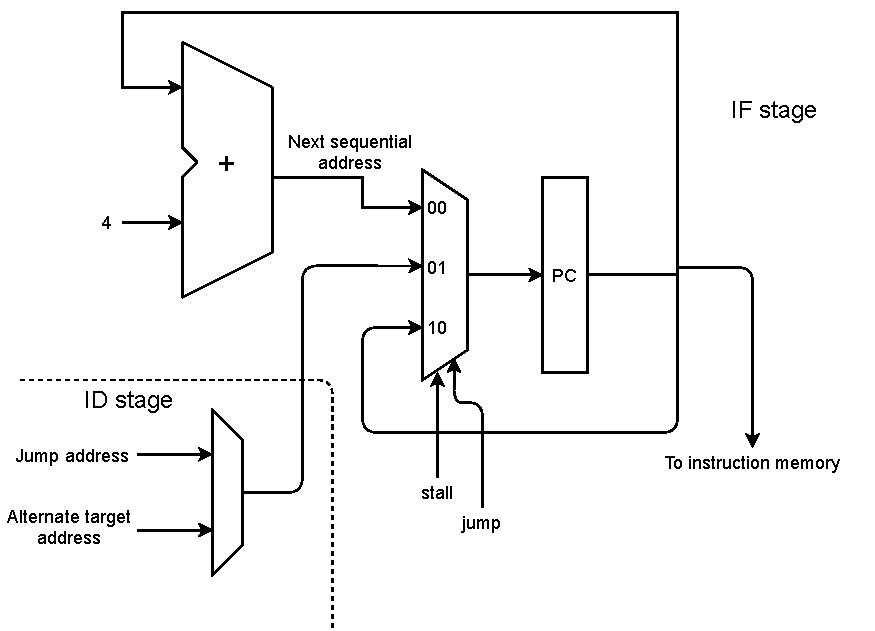
\includegraphics[width=0.6\textwidth]{../images/IF.pdf}
	\caption{RTL schematic of the instruction fetch stage, with part of the ID stage reported which selects the right jump address according to whether it is triggered by a jump instruction or a misprediction.}
	\label{fig:ifstage}
\end{figure}
\newpage
\section{Instruction decoding}
The instruction decoding step occurs just after the instruction is fetched from memory. Its purpose is to identify the operation to be performed, generating control signals for subsequent stages. Its tasks also include detecting particular execution states where the pipeline has to be stalled or flushed.
Given the variety of its purposes, this block is furtherly broken down into several sub-units hierarchically:
\begin{itemize}
	\item Decoder
	\item Hazard Detection Unit (HZU)
	\item Branch Prediction Unit (BPU)
	\item Target address computation
	\item Register File
\end{itemize} 

\subsection{Decoder} 
The simplicity of RISC instruction sets consists in including few instructions that perform simple tasks. Furthermore, the instruction format is fixed, so as to allow the decoding circuitry to be as simple and fast as possible. Five types of instruction are defined in RISC-V, with the following types of fields that could be present depending on the actual format:
\begin{itemize}
	\item Opcode
	\item Specialized opcode fields for arithmetic operations (funct3 and funct7)
	\item Destination register
	\item Source registers (one, two or none)
	\item Immediate field, whose size and format varies across types
\end{itemize}
Since the position of each of these fields is fixed, they can be extracted into separate signals without detecting the instruction type first. After instruction decoding, the relevant fields are used and invalid signals corresponding to inexistent fields are just ignored.

The main task of this sub-unit is to drive control signals for execution, memory and writeback stages, which includes part of the ID stage itself given that data is written back to the register file.

The VHDL description consists in a combinational process whose sensitivity list includes the opcodes and the source registers. Based on \texttt{rs1} and \texttt{rs2}, this unit will resort to the hazard detection unit to handle the load-use data hazard occurring when the source operand is to be loaded from memory within the following two clock cycles. Under this circumstance, an operation that depends on such operand cannot proceed to the execution stage because it will be too early for the required data to be available of forwardable. Whenever the HZU runs into a load-use data hazard, the decoding step produces a nop (no operation), meaning that all control signals are inactive and the instruction fetch stage is prompted to refetch the current instruction without updating \texttt{PC}. The normal execution flow proceeds as soon as the hazard is removed.

\begin{figure}[h]
	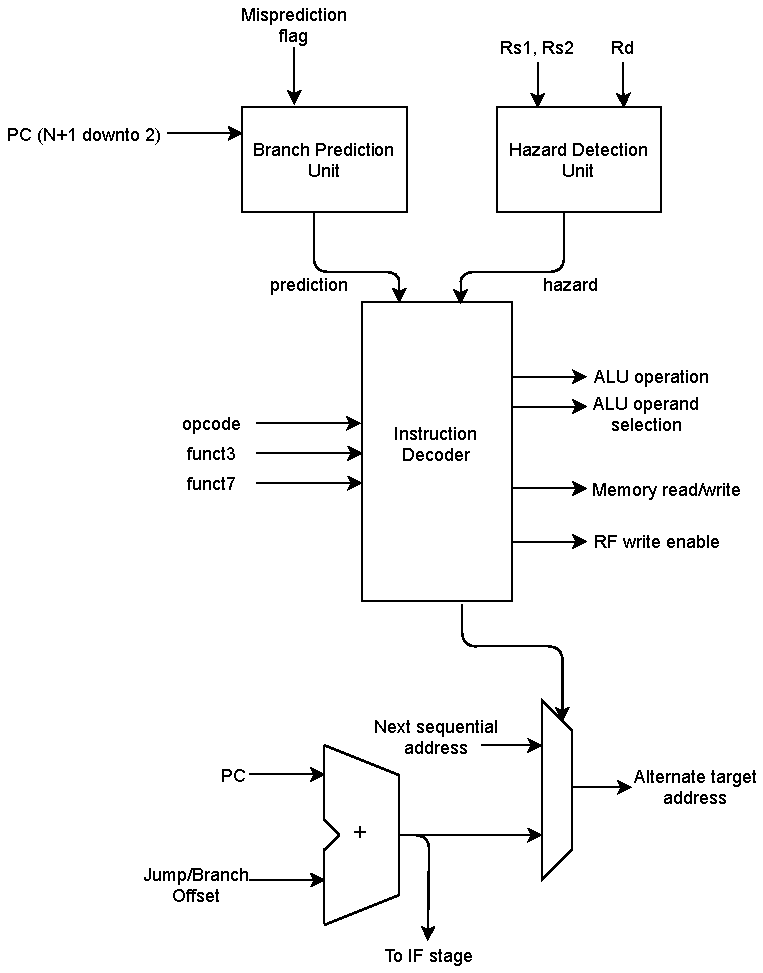
\includegraphics[width=0.6\textwidth]{./images/idstage.pdf}
	\caption{Instruction decoding stage with its sub-units}
	\label{fig:idstage}
\end{figure}

\subsection{Hazard Detection Unit} This subunit takes the source register indices and the \texttt{rd} signals (destination register name) both at the output of ID/EX and EX/MEM pipeline stages. If any of \texttt{rs1} or \texttt{rs2} is the same as \texttt{rd} and the corresponding data memory read enable signal is active, then the condition for a potential load-use data hazard is verified. The instruction decoder will trigger a nop insertion after validating the hazard signal coming from this unit, which is effective only if the instruction depends on the data contained in the register involved in the hazard.


\subsection{Branch Prediction Unit} The purpose of this block is to estimate which is the most likely path that the execution will take in case of branch instruction. The actual outcome of the branch condition is known as soon as \texttt{beq} reaches the MEM stage, which happens with a two clock cycles delay. The BPU uses this outcome to update its internal state according to algorithms specifically designed to refine the prediction accuracy by collecting execution statistics.

In our implementation, branches are statically predicted to be taken, in a similar way as prediction schemes used in early microprocessors. The introduction of a BPU influences the timing of the processor. With a BPU, the pipeline is stalled upon decoding a \texttt{beq} for only one clock cycle if the branch is predicted, the minimum required to jump to a non-sequential address. The actual execution path as determined by checking the \texttt{Z} flag is compared to the prediction only two clock cycles later by combinational logic contained in the MEM stage. A misprediction causes the pipeline to be flushed (pipeline registers are reset to a \texttt{nop} state) and the IF stage to jump to the alternative target address available in the EX/MEM pipeline register, which contains the alternative address computed in the ID stage.

A basic one-level scheme is the bimodal predictor, consisting in an array of 2-bit saturating counters addressed by part of the instruction address. Whenever a branch is decoded, the counter corresponding to its address is read, thus giving a 'taken' prediction when its value is greater than 1 and 'not-taken' otherwise. As soon as the real outcome of the branch is available the counter is incremented in case of a taken branch and decremented otherwise. This, in our implementation, occurs two cycles after decoding, when the branch is in the MEM stage. In general this delay, which affects the branch penalty to be paid in case of a flush, depends on the number of pipeline stages in between ID and MEM.


\subsection{Target address computation} This is accomplished simply by summing the offset specified in the instruction's immediate field (properly aligned and extended to 32 bits) to the current program counter. When the branch is predicted to be taken, this address is loaded in the pc and a jump takes place, with the next sequential address loaded in the alternative target address register. Otherwise, the TA is the alternative target address and the execution continues sequentially.

\subsection{Immediate} The immediate field is encoded differently depending on the instruction format. The ID stage takes care of aligning all the bits from the instruction word correctly and extending the sign bit to deliver a 32-bit immediate operand. This can take place after opcode decoding.

This is described in VHDL using a combinational \texttt{when-else} statement to synthesize a selection logic.

\subsection{Register file} As prescribed by the specifications, RV32I entails grouping 32 internal registers holding 32-bit data in a register file. \texttt{x0} denotes a location that always returns zero when read, thus making all write operations targeting it equivalent to not writing any data back.  

The VHDL description of this sub-unit is that of a standard memory, with additional care taken to obtain the correct synthesis for the \texttt{x0} location, which might not correspond to a physical register.
\newpage
\section{Execution Unit}
The Execution Unit is the unit responsible for the computations and the general execution of the commands.
The core and most significant component is the ALU, which the Execution Unit simply surrounds with multiplexers
and their controller to select the operands.

\begin{figure}[htbp]
    \center
	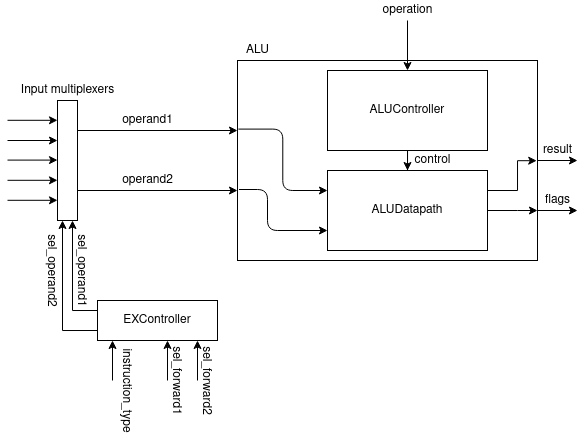
\includegraphics[width=0.8\textwidth]{./2-implementation/images/ExStage.png}
	\caption{Block view of the execution stage}
	\label{fig:exstage}
\end{figure}

\subsection{ALU}
The ALU is also internally organized with a datapath and its own controller. It is important to highlight that to not
interfere with the processor's pipeline, this controller (as well as the Execution Stage's) is fully combinational and
mostly acts as an input translator.

\subsubsection{Datapath}
The datapath instantiates the arithmetic and logic operators, generates the status flags and outputs the final result.
All the operators are instantiated in parallel and at every cycle, they all run their own operation and the result
is selected through a multiplexer. If power consuption is to be considered, guarded evaluation can be a simple
solution to this problem.

The available operators are:
\begin{itemize}
    \item Carry Look Ahead adder
    \item Barrel shifter
    \item And
    \item Xor
    \item Comparator
\end{itemize}

Most of their functionality is very straightforward: the \texttt{and} and \texttt{xor} operators are simple logic gates,
while the barrel shifter is described through the \texttt{numeric\_std} library's function \texttt{shift\_right} and
likely instantiated as a cascade of multiplexers. The components worth discussing are the adder and the comparator.

\paragraph{Adder}
The adder is designed as a \textbf{Ladner-Fischer} Carry Look Ahead.
\begin{figure}[htbp]
    \center
	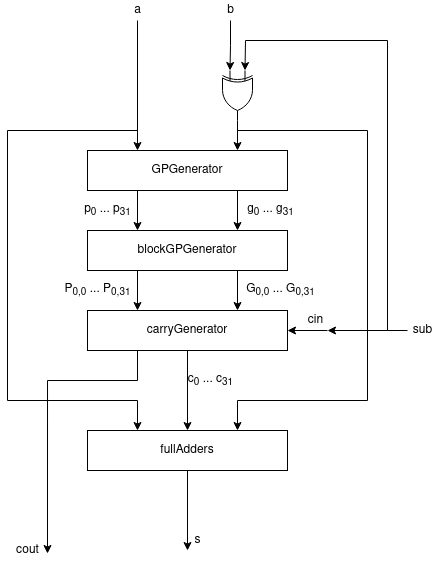
\includegraphics[width=0.5\textwidth]{./2-implementation/images/AdderCLADiagram.png}
	\caption{Carry Look Ahead adder organization}
	\label{fig:adder-diagram}
\end{figure}
Its structure is organized as a cascade of the following
blocks:
\begin{enumerate}
    \item Sign converter \\
    To accomodate for subtractions, operator \signal{b} goes through a \texttt{xor} gate controlled by the
    \texttt{sub} signal which, when asserted, also sets the \signal{cin} to 1.

    \item Generate and Propagate bits generator \\
    Given \signal{a} and \signal{b}, output the corrisponding generate and propagate signals bit by bit, where
    \begin{align*}
        g_i &= a_i\ \texttt{and}\ b_i \\
        p_i &= a_i\ \texttt{xor}\ b_i
    \end{align*}

    \item Block Generate and Propagate bits generator \\
    Starting from $g_i$ and $p_i$, compute the block generate $G_{0, i}$ and propagate $P_{0, i}$ as a parallel prefix
    problem. This is where the Ladner-Fischer structure is instantiated.

    \begin{figure}[htbp]
        \center
    	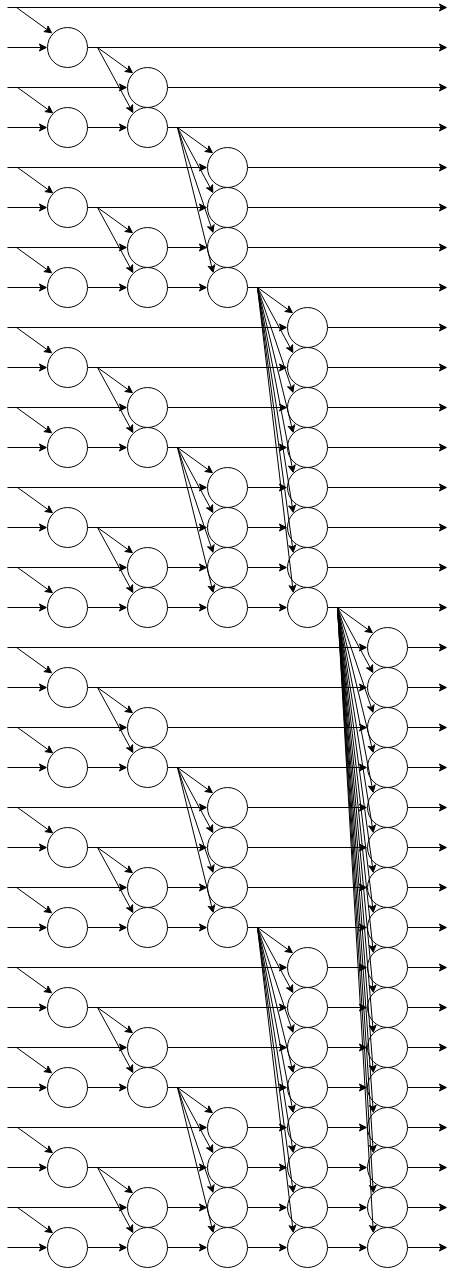
\includegraphics[width=0.5\textwidth]{./2-implementation/images/LadnerFischer.png}
    	\caption{Ladner-Fischer GPCombiner. Each circle represents an instance of the component GPCombiner.}
    	\label{fig:LadnerFischer}
    \end{figure}
    The main component needed to compute the block generate and propagate is called \texttt{GPCombiner} which, given
    $P_{i, j}$ and $P_{j, k}$, combines them into $P_{i, k}$ (and the same goes for $G$). The inputs $g_i$ and $p_i$
    (lowercase, meaning they are not the block generate and propagate but the bitwise ones) are assumed as $G_{i, i}$
    and $P_{i, i}$, which is equivalent. The operation is simple:
    \begin{align*}
        G_{i, k} &= G_{j, k}\ \texttt{or}\  \left( G_{i, j}\ \texttt{and}\ P_{j, k} \right) \\
        P_{i, k} &= P_{i, j}\ \texttt{and}\ P_{j, k}
    \end{align*}
    The combiners are connected according to the schematic in \autoref{fig:LadnerFischer} in the top level module,
    called \texttt{blockGPGenerator}. To keep the generality of the component, the block is described with generic
    and its structure is instantiated \textbf{recursively}. More information on the VHDL description can be found in
    \autoref{appendix:recursive-adder-description}.

    This is the slowest stage because it is the only one where chained combinational paths working on bits of different
    indices are needed. The choice of the Ladner-Fischer architecture makes so that the introduced delay is
    $\log_2{N}$.
    \item Carry Generator \\
    Given the results from the previous stage, it is possible to compute the value of all $c_i$ in parallel, since
    \begin{align*}
        c_i &= G_{0, i}\ \texttt{or}\ (c_0\ \texttt{and}\ P_{0, i})
    \end{align*}

    \item Full adders \\
    The final stage is a barrier of full adders. At this point, every adder has all of its inputs ready: $a_i$, $b_i$,
    $c_i$. For this reason there is no need for one adder to wait for the result of another adder, but they can all
    operate in parallel, so the introduced delay is only $1\ ^t\text{FA}$.

    \item Flag generators \\
    The adder also generates two overflow flags to be used to control the flow of operations: one for signed sums, one
    for unsigned ones. In particular,
    \begin{align*}
        \texttt{cout} = C &= c_{32} \\
        \texttt{ovf} = V &= c_{32} \texttt{ xor } c_{31}
    \end{align*}
\end{enumerate}
The ALU also internally computes all of the status flags: C and V are obtained directly from the adder, Z and N are
trivial to obtain by checking the sum result.

\paragraph{Comparator}
A comparator is usually implemented as a subtractor that then performs some checks on its result, given that the generic
comparison operation $?$ between $A$ and $B$ can be expressed as
\begin{align}
    A\ ?\ B &\rightarrow A - B\ ?\ 0
\end{align}
Since an adder/subtractor is already available and all of the relevant observations on the result were performed for
the status flags, the comparator is implemented as an extension of the adder that only checks the status flags and
outputs a result based on the requested comparison.

It internally computes all of the possible comparisons and a multiplexer selects the result to output. In particular,
\begin{align*}
    lt &= N \texttt{ xor } \texttt{overflow} \\
    le &= lt \texttt{ or } Z \\
    eq &= Z \\
    ge &= \texttt{not } lt \\
    gt &= \texttt{not } le
\end{align*}
The \texttt{overflow} signal is either C or V, depending on whether the comparison should consider its operands as
respectively unsigned or signed.

It is clear to see how it is the controller's job to correctly deliver all of the necessary commands when a comparison
is requested, such as switching the adder to subtracting mode, deciding whether the operands are signed or not and
selecting the otuput.

\subsubsection{ALU Controller}
The controller for the ALU receives an ALU opcode to choose what operation to perform and then internally manages all
the necessary signals. It is described with a simple process and a switch on the opcode that updates the control
signals, as in any classical control unit output process.

For example, when the opcode is \texttt{alu\_op\_lt}, the control unit sets \texttt{adder\_sub} to 1 (to perform a
subtraction instead of an addition), switches the ALU multiplexer to select the comparison result, specifies to the
comparator that the data is signed and switches its multiplexer to choose the \texttt{lt} result.

All of the control signals are packed inside of a VHDL record to simplify possible future changes without the need of
modifying any entity in the circuit.

\subsection{Input Selection}
sdasadsdasa

\newpage
\section{Adding ABS}
\newpage
\section{Forwarding Unit}

 Forwarding unit is a unit that works across Execution stage, Memory Stage and Write-back stage. Its role is to prevent read after write data hazard that can occur between successive instructions due to the pipelined implementation of the processor. To do so, it compares separately the source register Rs1 and Rs2 of the instruction at Execution Stage first against destination register Rd of the instructions at Memory Stage, then against the one of the instruction at Write-back stage. If there is a match it checks also that this register is not x0, and that the destination register will be effectively wrote-back into the register-file, otherwise the forwarding will be useless or wrong.
 
 Performed all the comparisons, the Forwarding unit tells to the execution if the correct operands are to be taken from register-file, Memory Stage or Write-back stage. 

\newpage

\chapter{Verification}
\section{Instruction decoding}
This sub-unit was tested along with the rest of the pipeline, since several signals coming from other stages are important to determine the control flow. For instance, the misprediction flag is generated in the MEM stage and the data used by the hazard detection unit comes from the pipeline registers. The instruction decoding stage was connected to a behavioral ALU in order to focus the debugging effort on the instruction sequence. \autoref{fig:wave} shows the occurrence of a branch (at $t=1.2\, \mu$s), the corresponding jump due to the taken prediction and the subsequent recovery two clock cycles later, when the prediction is found to be incorrect.

\begin{figure}
	\makebox[\textwidth][c]{
	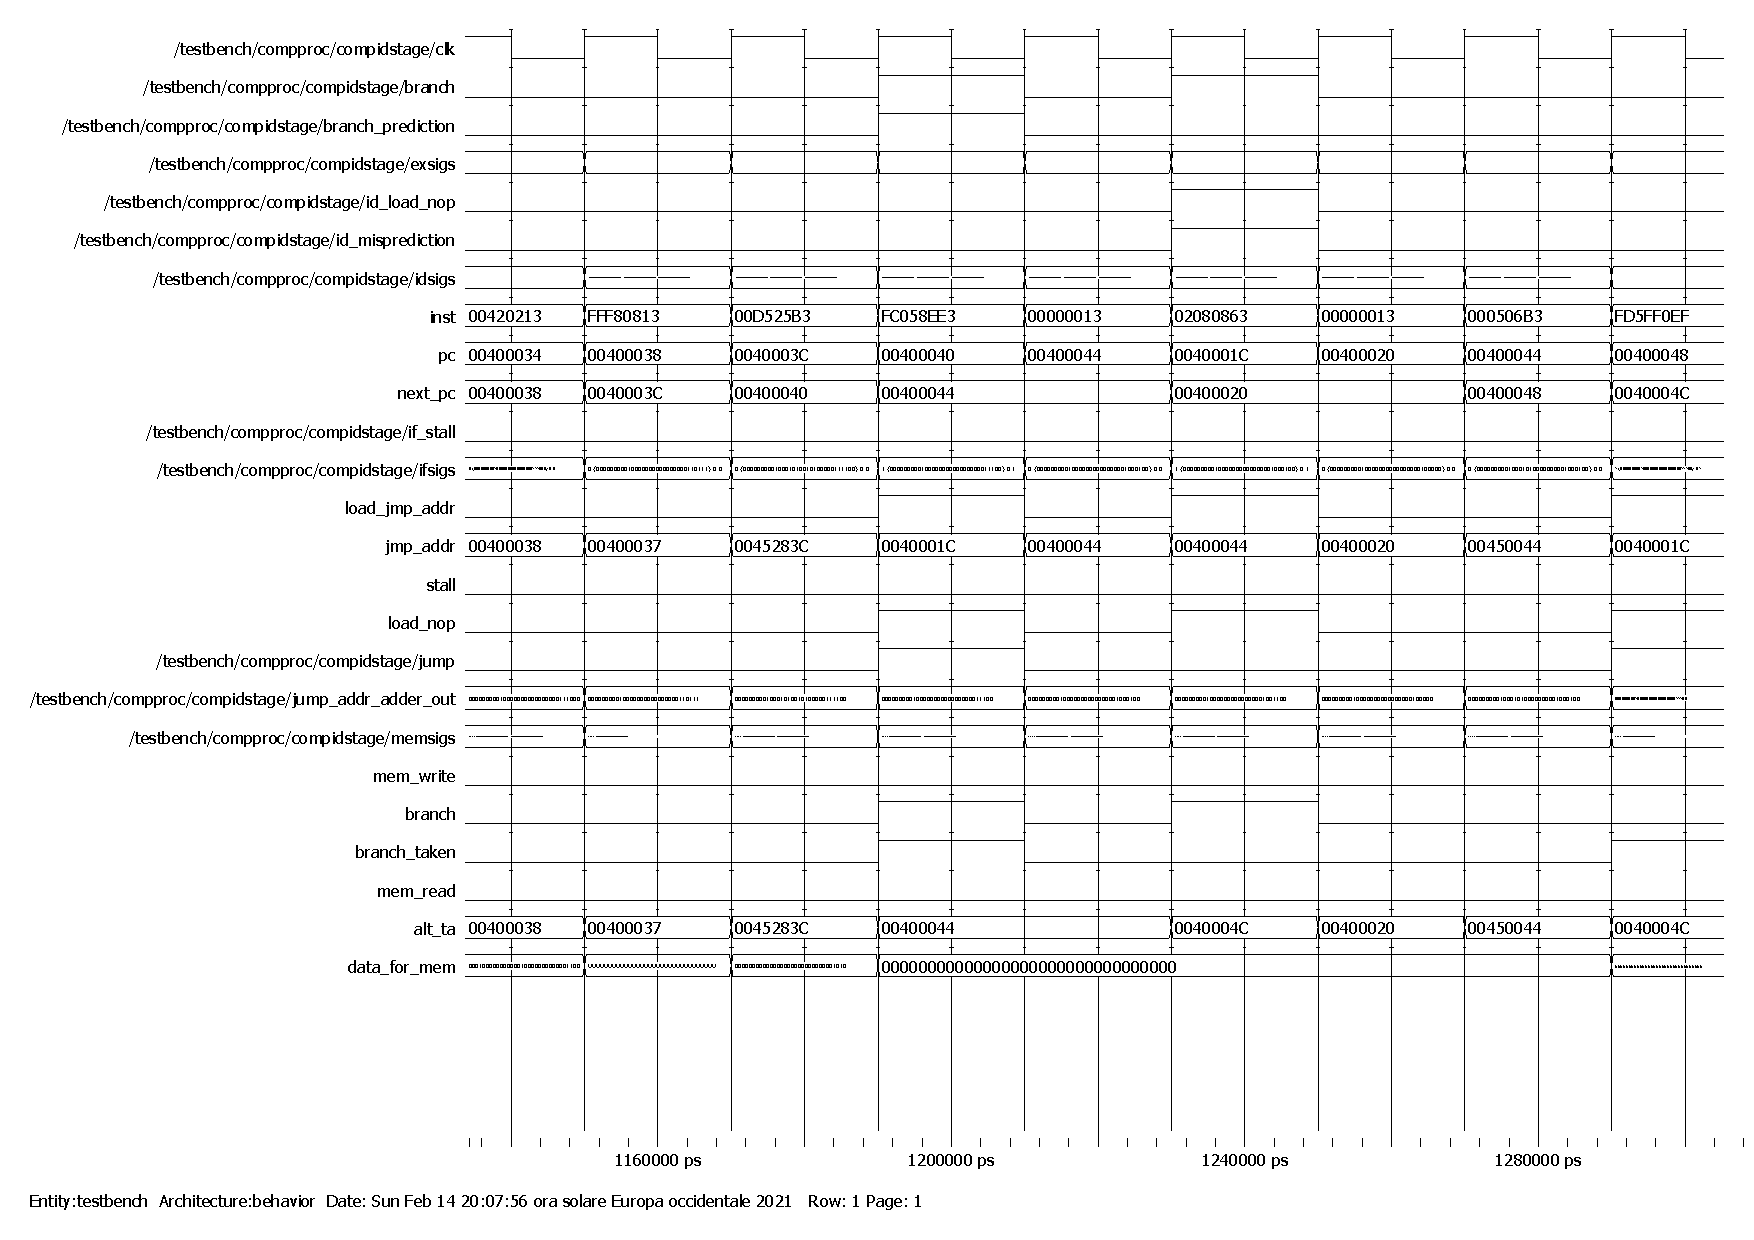
\includegraphics[angle=90, width=1.2\textwidth]{./images/wave.pdf}}
	\caption{Instruction decoding stage signals showing the occurrence of a branch and the following flush due to its misprediction.}
	\label{fig:wave}
\end{figure}


\section{Execution Stage}
The most significant component to verify is the ALU.

\newpage

\chapter{Synthesis}
\section{First version}
\begin{table}[h]
	\centering
\begin{tabular}{|l|l|l|}
	\hline
	& \texttt{compile} & \texttt{compile\_ultra}\\\hline
	Area & 15500 & 14800 \\\hline
	$T_{ck}$& 1.14 ns & 1.10 ns\\\hline
\end{tabular}
\caption{Comparison between standard and ultra compile}
\label{tab:comp}
\end{table}

\paragraph{Maximum clock frequency} The basic design was synthesized with the retiming option enabled using both the standard compile followed by \texttt{optimize\_registers} and \texttt{compile\_ultra}. \autoref{tab:comp} shows that in this case the second option should be preferred. The compiler issues a warning when it applies retiming to registers that have both a preset and a reset signal, a situation that occurs with pipeline registers since they must be initialized at startup and reset synchronously during the execution as well (flush). Therefore, a simulation of the synthesized netlist is mandatory to verify that the retiming has not altered the functionality of the processor. This check was done on the testbench program provided (minimum search) with successful results.

\paragraph{Final synthesis} After the zero clock period synthesis, a second compile command was issued with a slightly larger clock period constraint in order to obtain the final netlist to be routed. The results of this process are summarized in \autoref{tab:synres}. The QOR report indicates that there are as many as 20 logic levels, this suggests that this design could benefit from a deeper pipeline, since it is well known that the ideal number of combinational logic levels for a processor is between 6 and 8.

The result from \texttt{report\_resources} indicates that several DesignWare library components were used to synthesize comparators, incrementers and decrementers in the IF and ID stages. A barrel shifter was inferred in the ALU and an incrementer/decrementer in the branch prediction unit.

\begin{table}[h]
	\centering
	\begin{tabular}{|l|l|}
		\hline
		Area & 14644 \\\hline
		Combinational area & 7438 \\\hline
		Noncombinational area &7205\\\hline
		Clock period & 1.16 ns \\\hline
		Critical path length & 1.05 ns\\\hline
		Levels of logic & 20 \\\hline

	\end{tabular}
\caption{Synthesis results}
\label{tab:synres}
\end{table}

\chapter{Conclusion}

\end{document}
